% Chapter 3 from the thesis template file
%   that contains an example table and figure.

%Chapter 3: Background
%1) Introduction paragraph summarizing the flow/content/structure of the Background chapter
%2) Radiometer Basics
%	a) Power Detection
%	b) Integration and filtering
%	c) Metrics
%		i) Sensitivity
%		ii) Stability
%	d) Implementation
%3) Software Defined Radio Basics
%	a) High-level figure of the components of a generic SDR.
%	b) SDR Operation
%	c) GNURadio Operation
%4) Software Defined Radio Development Platform (i.e. your specific platform)
%	a) Hardware (i.e. N200)
%	b) Software (i.e. GNU Radio)  

\chapter{BACKGROUND}\label{ch:background}

This chapter will examine background information on the basic operation of a radiometer, a software defined radio and background on the development platform used to build a software defined radiometer.  We begin with an overview of a traditional radiometer and how this type of radiometer works.  This is followed by high level examination on how a software defined radio operates.  Finally we will discuss both the hardware and software selected and used for our development platform to create this software defined radiometer.

\section{Radiometer Basics}

The primary task of a radiometer is to measure power.  While that statement sounds easy, there are many factors that go in to how well a radiometer can measure the power it observes.  A better statement is that a radiometer's primary goal is to accurately measure the correct power within a certain degree of accuracy.  In order to accurately and within a high degree of precision measure power a radiometer must take into account factors such as the system noise, the bandwidth of the signal and the stability of the system as a whole[\cite{Evans}].  

%The amount of noise that is generated by the object of interest is due to the thermal agitation of the charge carriers, usually the electrons, which is directly correlated to the physical temperature of the source[\cite{Nyquist1928thermal}].  This correlation is done as a noise temperature.  All objects emit this noise and the intensity will vary on multiple parameters and on what the source is.  One source that has current research at Iowa State University is in detecting soil moisture.  Numerous soil types can be observed including sandy types of soil[\cite{Liu}], The brighter or warmer the noise temperature is, the more RF noise that has been received which correlates to a drier soil.  The less RF noise power received the cooler the noise temperature and this indicates wetter soil area. Radiometers such as these are already in service on satellites such as the Soil Moisture and Ocean Salinity (SMOS) satellite launched by the European Space Agency (ESA) and are used by scientists to monitor the Earth's soil moisture and ocean salinity[[\cite{McMullan}][\cite{Hardy}].  

In all radiometers there are six stages that is common in all radiometers.  They are:

\begin{enumerate}
\item Source (antenna or $T_{A}$)
\item Amplification (Gain or $G$),
\item Bandwidth restriction (filtering or $\beta$),
\item Power detection ($X^{2}$),
\item Integration ($\tau$),
\item Output.
\end{enumerate}

Figure \ref{trad_radiometer} shows each stage as they relate to each other.  We begin with our source which is often an antenna.  Amplification or gain in the system then amplifies this signal so that it is easier to measure changes in our noise.  Filtering can occur before or after the amplification stage and in some cases filtering is done before and after the filtering stage.  Power detection extracts the power information from the signal.  Because the signal is often noisy, we use integration to smooth our signal and improve our sensitivity.  Finally our output is the total power information.  This information may be as simple as a voltage output or may be a calibrated noise temperature.

{\begin{figure}[h!tb] 
\centering
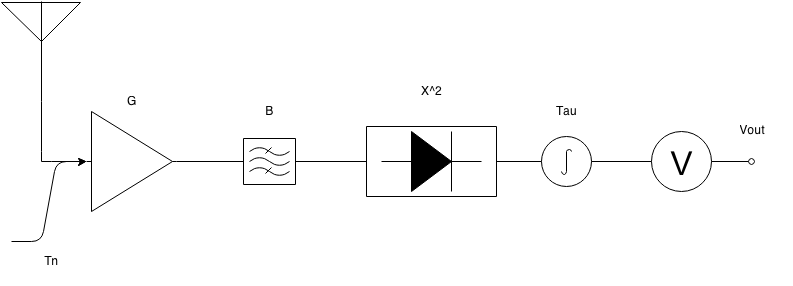
\includegraphics[width=\textwidth]{Images/Radiometer.png}
\isucaption{A total power radiometer block diagram}
\label{trad_radiometer}
\end{figure}
}

In figure \ref{trad_radiometer} we have one more component that is common in all radiometers but is not a physical component or stage in the radiometer.  That item is additional noise that gets added to the system from within the system itself is called system noise or $T_{N}$.

In addition to the system noise, another very common problem with radiometers is stability.  Most instabilities in a radiometer are due to fluctuations that occur in the amplification stage or the Low Noise Amplifiers (LNAs) used. These gain fluctuations can be controlled to a point by closely monitoring and controlling both the voltage and the temperature of the LNAs. However, this is not an easy task and in some cases is not practical.  Therefore, other methods have been developed to compensate for these fluctuations.  There are three common types of radiometers designed to adjust for gain fluctuations.  They are:

\begin{enumerate}
\item Dicke radiometer,
\item Noise injection radiometer,
\item Polarimetric or correlating radiometer.
\end{enumerate}

%Additional noise in the system is impossible to eliminate, however we can take steps to reduce it as much as possible.  In addition, we can calculate what this noise is and take steps to account for it in our measurements.  However, this means that stability is another parameter within the radiometer.  If the noise generated within the radiometer is constantly changing then this makes it difficult to account for this additional noise.  

One of the first methods used is the Dicke radiometer which switches between the measurement of the antenna and a known source[\cite{Dicke}].  By referencing this known source very quickly the Dicke radiometer can account for and greatly reduce gain fluctuations.  

{\begin{figure}[h!tb] 
\centering
\includegraphics[width=\textwidth]{Images/Dicke_block.png}
\isucaption{A block diagram of a Dicke radiometer}
\label{dicke_radiometer}
\end{figure}
}

While a Dicke radiometer greatly reduces the fluctuation in the gain of the radiometer and improves stability, it does so at the cost of not seeing the object of interest while it is referencing the known source.  This decreases the sensitivity of the radiometer.

{\begin{figure}[h!tb] 
\centering
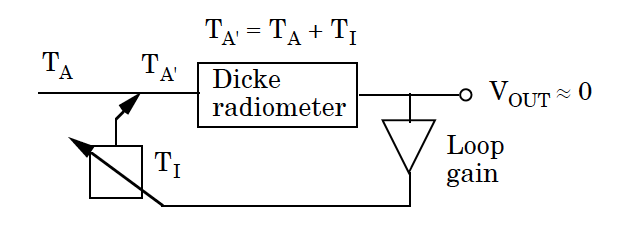
\includegraphics[width=\textwidth]{Images/NoiseInj_block.png}
\isucaption{A block diagram of a Noise Injection radiometer}
\label{NoiseInj_radiometer}
\end{figure}
}

A noise injection radiometer is a variation of the Dicke radiometer where a variable noise source is used and injected into the RF chain as seen in Figure \ref{NoiseInj_radiometer}.  The output of this noise source is then adjusted so that the noise input plus the signal from our source is equal to the reference noise.  This completely eliminates fluctuations however increases the system noise which also reduces our sensitivity of the radiometer.

Our source signal is often times assumed to be not polarized.  However, this is not the case and an incoming signal often has some polarization.  A correlating radiometer [\cite{Fujimoto}] uses a dual polarization antenna to split the vertical and horizontal polarization of the signal.  Each of these signals is then fed into a radiometer and our correlated.  Since gain fluctuations or uncorrelated, they are reduced in the system.  This reduces gain fluctuations and also helps maintain the sensitivity of the radiometer.  However it adds a much greater complexity to the radiometer and requires two identical receivers.  

%Additional improvements to radiometers have also been done by digitizing parts of the radiometer.  The most common method for doing this is by digitizing the analog output of the square-law detector and sending that to a computer or processing unit to analyze the data[\cite{Bremer}].  While this does allow for easier computation and storage of the information it does not alleviate the needs to maintain stability or reduce possible additional noise of the system since this data is digitized after the RF signal chain.

\subsection{Measuring RF power}

To measure power in a radiometer, several factors are taken into consideration.  To begin with we have the noise signal coming from the antenna.  Our antenna is assumed to be looking at our target of interest and it is assumed that we can relate the antenna noise to the noise from the source.  It is often easier to refer to this noise as the brightness temperature.  Therefore, the brightness temperature of the source can be related to the brightness temperature at the antenna.  We will refer to this brightness temperature as $T_{A}$.  

{\begin{figure}[h!tb] 
\centering
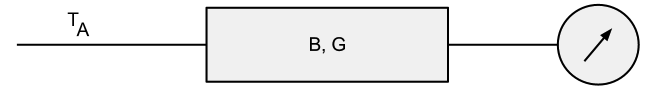
\includegraphics[width=\textwidth]{Images/simple_rad.png}
\isucaption{The ideal radiometer block diagram}
\label{simplerad}
\end{figure}
}

Figure \ref{simplerad} shows us an ideal radiometer.  That is a radiometer that has an input from the antenna, $T_{A}$, a known bandwidth denoted as $B$ or $\beta$ and a known gain denoted as $G$.  At the end of the block is the detector, which measures the power from the radiometer.

%Only a certain selection of the radio spectrum is observed by the radiometer and this is the bandwidth of the radiometer.  In our scenario, we center around 1.4125 GHz.  There is a reason why 1.4125 GHz is selected and that is from 1.4000 to 1.4250 GHz is protected internationally to be as radio frequency interference free as possible.  This reduces interference from outside sources such as transmitters that can interfere with the operation of the radiometer.  

The power coming from the antenna is the combination of the following items:

\begin{enumerate}
\item Gain or $G$ of the system,
\item Bandwidth or $\beta$ of the system,
\item Signal source or $T_{A}$.
\end{enumerate}

To calculate our power from the radiometer, we multiply each item with the Boltzmann constant referred to as \textit{k}. Equation \ref{eq:power_rad_eq} gives us the total power, in watts, of an ideal radiometer.

\begin{equation} \label{eq:power_rad_eq}
P=k*\beta*G*(T_{A}) (watts)
\end{equation}

As discussed in the above section, the system noise is another component of the radiometer that needs to be addressed.  Figure~\ref{noiserad} shows the additional noise that is injected into the system.

{\begin{figure}[h!tb] 
\centering
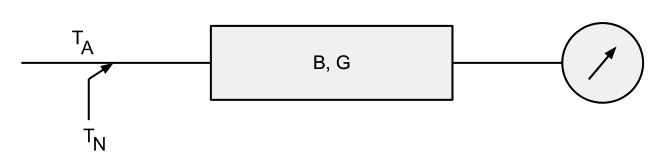
\includegraphics[width=\textwidth]{Images/radiometer_noise_added.png}
\isucaption{A more realistic radiometer model}
\label{noiserad}
\end{figure}
}

As it can be seen, this additional noise is added to the noise coming from the antenna source.  Therefore, T$_{N}$ is added to T$_{A}$ and our final equation for the power measured is shown in equation~\ref{eq:final_power}.  

\begin{equation} \label{eq:final_power}
P=k*\beta*G*(T_{A}+T_{N}) (watts)
\end{equation}

Figure \ref{trad_radiometer} showed us a more typical radiometer and was discussed in the previous section.  However, power detection and the associated voltage output has not been discussed.  Power detection is accomplished typically with a square-law detector and this output is often run through an integrator to smooth the output[\cite{Leinweber}].  Finally we have the output which is a voltage represented as V$_{out}$.  This results in equation~\ref{eq:vout_1}.

\begin{equation} \label{eq:vout_1}
V_{OUT}=c*(T_A+T_N)*G
\end{equation}

Here V$_{OUT}$ is shown by the addition of both the noise from the system T$_N$ and the noise from the antenna, T$_A$ and multiplied by the gain in the system, $G$ [\cite{skou}].  A constant factor $c$ is useful for when we are looking at a radiometer like a Dicke radiometer in which the value of $c$ is $\frac{1}{2}$.  In most applications outside of a Dicke radiometer, $c$ is 1 and can be ignored.  

The voltage output from this radiometer is then either measured or may also be sampled by an analog to digital converter.  This voltage then represents the total power measured by the radiometer, however this measurement is not calibrated.

%Most radiometers are more complicated than the one shown in Figure~\ref{noiserad}.  Additional signal conditioning is often needed which filters and may also amplify or attenuate the signal as required for proper performance through the RF chain.  Once the total power is detected a method to measure and store this reading must also be done.  Finally, additional hardware may be required to stabilize the radiometer which will be discussed in more detail in this thesis.

\subsection{Integration and filtering}

Filtering with a traditional radiometer is usually accomplished by using mechanical filters.  Often these are band-pass filters that limit the bandwidth that the radiometer sees.  Other filters, such as a low pass filter are also used, but usually to smooth out the output from the square law detector.  Another item used to help smooth out the signal from the square law detector is an integrator.

A RC filter is analogous to an integrator where the R and C values determine our time constant and our integration time for the filter[\cite{Aitken}].  We know a RC filter is analogous to an integrator by looking at equation \ref{eq:rc_int}.

\begin{equation}\label{eq:rc_int}
\frac{1}{RC}\int{V_idt}
\end{equation}

To begin with, we look at what an analog RC filter looks like. 

{\begin{figure}[h!tb] 
\centering
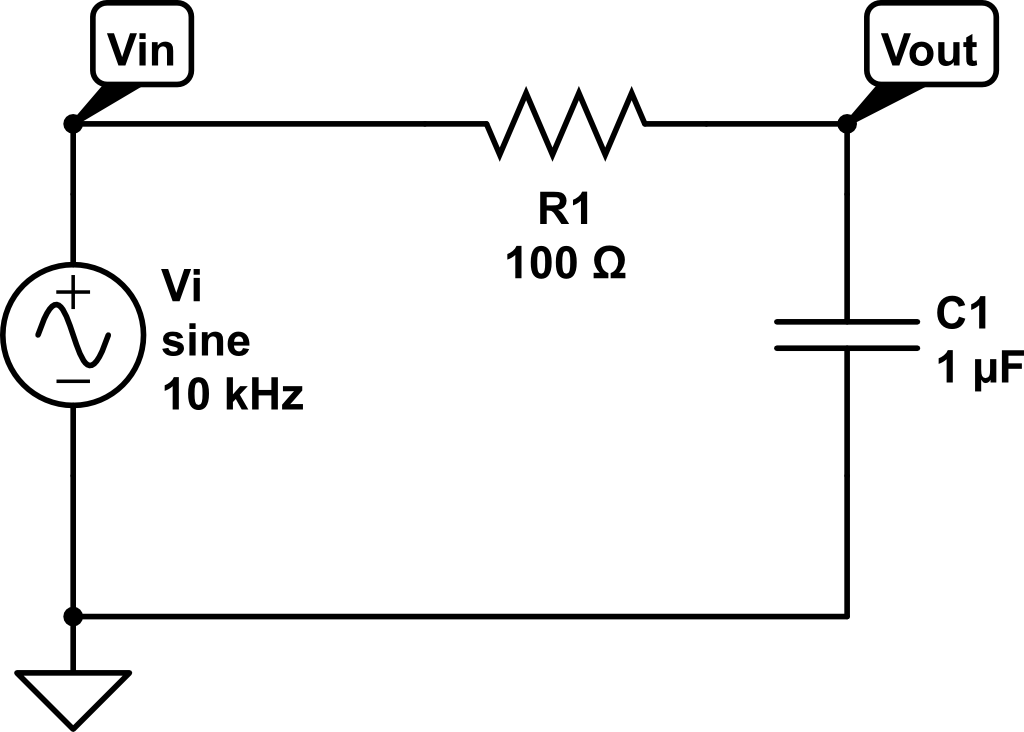
\includegraphics[width=10cm]{Images/rc-circuit.png}
\isucaption{A simple RC circuit}
\label{rc_circuit}
\end{figure}
}

This circuit can be represented by equation \ref{eq:rc_circuit_eq}.

\begin{equation}\label{eq:rc_circuit_eq}
\frac{V_{in}-V_{out}}{R}=C\frac{dV_{out}}{dt}
\end{equation}

This integration smooths out the signal from the square law detector and also improves our sensitivity of the radiometer.  This will be further explained the next section.

\subsection{Radiometer Performance Metrics}
There are two criteria that determines how well a radiometer performs.  The first criteria is with the sensitivity of the radiometer.  This tells us how well the radiometer can differentiate between the information we want and the noise we do not want.  The second criteria is stability.  A radiometer needs to be calibrated to give us useful information.  Stability refers to how much change or drift a radiometer is experiencing which in turn can affect the accuracy of our data.  

\emph{Sensitivity}.  Sensitivity of the radiometer relates to the amount of power that the radio selects from the antenna.  This selection is then dependent on the bandwidth that the radiometer is able to listen to.  The radiometer however detects not only the signal of interest but also receives a noise signal as well.  This noise is added to the signal and can not be separated from the signal.  Because this noise is added to the signal, we must be able to determine a change in the signal while the noise signal is also present.  

To understand this, let us look at the example of T$_{A}$ has a value of 200 K and T$_{N}$ has a value of 800 K.  Since T$_{N}$ is added to our antenna signal, we have a total noise temperature of 1,000 K.  This means that if we want to detect a change as small as 1 K, we must be able to measure the difference between 1,000 K and 1,001 K[\cite{skou}].

%Equation \ref{eq:final_power} shows us the total power from the radiometer, where we take into consideration bandwidth, gain and the input from the antenna plus the noise added from the antenna.  

The ability of a radiometer to detect these small changes is the radiometer's sensitivity, or the standard deviation of the output signal from the radiometer.  This sensitivity is also referred to as the Noise Equivalent Delta ($\Delta$) Temperature or NE$\Delta$T and is shown in equation \ref{NEAT_EQ}. 

\begin{equation} \label{NEAT_EQ}
NE\Delta T=\frac{T_{A}+T_{N}}{\sqrt{\beta * \tau}} 
\end{equation}

The sensitivity of the radiometer is based on both the bandwidth, $\beta$, of the incoming signal and the integration time, $\tau$.  As it can be seen in the equation, we want to have as much bandwidth as possible.  In a traditional radiometer, this bandwidth is often fixed and is dependent on the band-pass filters used in the radiometer.  We can however control $\tau$ and a longer integration time will help improve the sensitivity of the radiometer to a certain degree.[\cite{ulaby}]

\emph{Stability.}  Stability and accuracy are additional problems that need to be considered when looking at the radiometer system.  To begin we can once again look at the power received equation \ref{eq:final_power}.

As we look at this equation, we can see that if $k$, $\beta$, $G$, and $T_{N}$ are constant, then stability can be assured.  The Boltzman constant $k$ is a known constant and we can also assume that our bandwidth, $\beta$, will also remain constant.  Gain and the noise temperature however will vary.  

Fluctuations in gain is the largest factor that affects stability in the system and this can be seen in equation \ref{eq:rad_stability}.  As discussed earlier, it is this factor that has been a driving force for changes to the design of a radiometer as demonstrated by the Dicke and Correlating radiometer designs.  

Gain fluctuations are caused by two factors: the physical temperature of the amplifier and the voltage that feeds the amplifier.  High accuracy voltage regulators can help control fluctuations in voltages that can in turn affect the gain.  A factor however that is harder to control is temperature.  Various methods have been used to control the temperature when the radiometer is used in fluctuating temperature environments such as the outdoors or in space.  

\begin{equation} \label{eq:rad_stability}
\Delta T_G=T_{sys} \left(\frac{\Delta G}{G}\right)
\end{equation}

With stability we need to either attempt to stabilize the radiometer as best as we can or compensate for the gain fluctuations.  Compensation has been discussed and three types of radiometers have been identified that attempt to compensate for these fluctuations.  To control the stability many radiometers will use highly accurate voltage regulators and will control the temperature of the LNA through methods such as thermal electric coolers.

%\subsection{Implementation of traditional radiometer}
 
\section{Software Defined Radios Basics} 
The basic concept behind a SDR is that it will digitize the RF signal as soon as possible.  Once digitized, it is now evaluated by a computer, FPGA, or a dedicated System on Chip (SoC).  A canonical software defined radio architecture is one that consists of a power supply, antenna, multi-band RF converter, and a single chip that contains the needed processing and memory to carry out the radio functions in software [\cite{Mitola1995}]. This allows us to extract certain hardware functions, such as filtering, into the digital domain which can then be manipulated by software.  Since software is now manipulating the signal, we can rapidly change what functions we execute on the signal by changing the software.  This gives SDRs a high amount of flexibility as components that are normally done in hardware can now be done in software and can be changed by simply uploading new software or firmware to the system.  This also gives us a benefit in cost as certain components are no longer needed and changes done in software do not require additional hardware to be added or to be swapped out.

An ideal software defined receiver simply has an antenna connected to an analog to digital converter which sends information to a processing unit such as a Field Programmable Gate Array (FPGA) or computer.  For a transmitter, we reverse it and use a digital to analog converter to produce the correct waveform which is then transmitted by the antenna.  In reality, SDRs require some additional hardware to make a viable working transceiver.  Amplification is still required to amplify the incoming signal and to amplify the signal going to the antenna.  Some SDRs also use a mixing stage to move a high frequency signal to a lower frequency signal.  This allows for less expensive analog to digital and digital to analog converters to be used.  

\subsection{Software Defined Radio Normal Operation}
Software Defined Radios (SDRs) are used for a variety of applications but their primary application has been in the area of communications.  They appeal to applications where being able to change a modulation scheme or filter on the fly is desirable.  In these areas, SDRs often outperform a traditional hardware only radio with their ability to rapidly change their operations by simply changing their software.  Early SDRs were expensive due to the high costs in the analog to digital converters (ADCs) needed and in the high speed Field Programmable Gate Arrays (FPGA) used.  In recent years however, the cost of SDRs have decreased due to the cost of these key components decreasing in cost as well.  Even though the cost has gone down the performance of SDRs have increased and this has lead to new developments in applications for using SDRs in new and different ways.

Software defined radios have been used in a number of applications.  Some applications they have been used in are:

\begin{enumerate}
\item Cellular communications,
\item Wireless local area networks,
\item Personal area networks,
\item Digital broadcast.
\end{enumerate}

There are of course other applications than those listed and more applications added as new communication methods continue to evolve [\cite{jondral2005software}].  But this is the strength of a software defined radio, it is capable of performing all of these operations and can be adapted to new ones by simply updating the software that defines it.

\section{Software Defined Radio Development Platform}
The work of this thesis is to use an off the shelf software defined radio (SDR) to perform the same operation or better of a traditional analog radiometer.  Using a SDR radio also means that we are able to be more flexible in how the radiometer performs, is capable of frequency agility and adapting to changing conditions such as interference.  Using a software defined radio also allows for implantation of different radiometer types such as a correlation radiometer or a polarimetric radiometer that uses Stokes parameters [\cite{Wang}].  Normally, these require changes to hardware, but all of these types of radiometers can be implemented in software increasing the flexibility of the system.  

\subsection{Hardware Platform}
The key component for a software defined radio radiometer is the hardware that will do most of the work of sampling and processing the signal.  The equipment selected for this work is the Ettus Research Group N200 SDR and can be seen in figure \ref{N200}.  The N200 has the following features that made it well suited for our specific application:

\begin{itemize}
\item Dual 14-bit ADC,
\item 50 MS/s Gigabit Ethernet streaming,
\item Modular daughter-board system for RF front end
\end{itemize}

This SDR utilizes daughter boards as the RF front end to the SDR and up to two daughter boards may be installed into a N200.  Another important reason the N200 is selected was due to its ability to handle up to 50 MHz of bandwidth to the computer and up to 25 MHz of RF bandwidth per daughter-board plugged in to the SDR.  This means that it is possible to have two receive cards that can stream up to 25 MHz bandwidth each.

{\begin{figure}[h!tb] 
\centering
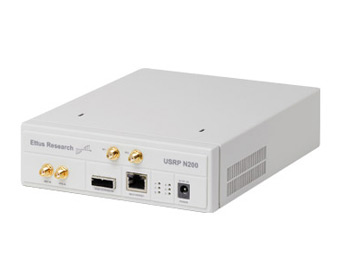
\includegraphics{Images/n200}
\isucaption{The USRP N200 from Ettus Research (Image from Ettus Research Website - www.ettus.com)}
\label{N200}
\end{figure}
}

The N200 utilizes a flexible architecture through the use of daughter-boards for a variety of RF interface systems based on the frequency range desired and if receive and/or transmission is needed.  Figure \ref{N200_block} shows the overall architecture of the N200 SDR.  These daughter boards directly receive the RF signal and then outputs the analog I and Q signals that are then sampled by the N200 A/D converter for reception or receives the I and Q values from the N200 D/A converter for transmission. 

{\begin{figure}[h!tb] 
\centering
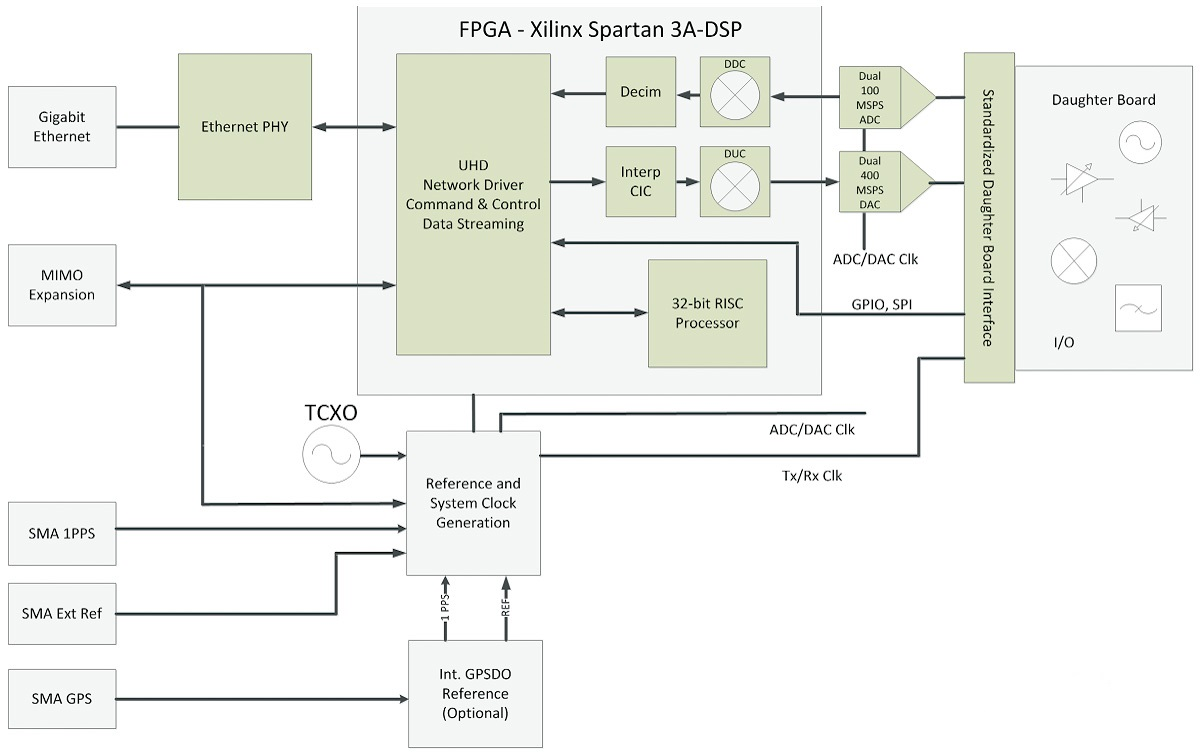
\includegraphics[width=14cm]{Images/n200_block_edited}
\isucaption{A block diagram of the Ettus N200 SDR. (Image from Ettus Research Website - www.ettus.com)}
\label{N200_block}
\end{figure}
}

The flexible architecture of the N200 and the ability for it to handle large amounts of bandwidth made this hardware ideal for the software defined radio radiometer work done in this thesis.

%These specifications had a large impact on the selection of the N200 for this application.  Specifically the 14-bit ADC, the 50 MS/s and the modular daughter-board system were the largest factors in the decision to use the N200 SDR.  Further explanation on these specifications are explained in the following sections.

%\emph{14-bit ADC.}  The analog to digital converters (ADC) allow us to take the analog I and Q values from the daughter boards and digitize this information.  Once digitized, we can now work with the signal both on the on-board FPGA board or stream it to the computer so that our software can manipulate the signal.  In radiometry, we are primarily looking at the overall power of the signal and this does not require us to accurately recreate the signal.  However, as will discuss later there are times were we do want frequency information and having an accurate frequency representation of the signal will then be an important factor.

%\emph{50 MS/s Bandwidth.}  The N200 is capable of working with up to 100 MS/s signal and can stream up to 50 MS/s through the Gigabit Ethernet connection.  The N200 also has the ability to have up to 2 daughter boards installed.  If we assume each will have up to a 20 MHz signal, this means up to 40 MS/s of data will be required.  This means that the N200 meets and can exceed the bandwidth requirements that we were looking for.  In addition, the FPGA on the N200 is capable of working with up to 100 MS/s, so there is room in handling additional bandwidth by using the on board FPGA to process the signal.

%The daughter board selected is the DBSRX2 card as this card is receive only and operates between 800 MHz and 2.4 GHz.  The DBSRX2 also has built in amplification that is adjustable through software.


\emph{The DBSRX2 Receiver.}  The daughter board selected is the DBSRX2 card as this card is receive only and operates between 800 MHz and 2.4 GHz.  An image of the daughter-board can be seen in figure \ref{dbsrx2}.  The DBSRX2 also has built in amplification that is adjustable through software.  These daughter boards have the required RF hardware for the signal to be processed.  In this application it was required that the signal was detected at 1.4 GHz with a bandwidth of 20 MHz.  The DBSRX2 receiver met this requirement and was selected to be used with the N200.  In this radiometer application transmission is not needed and is illegal in the 1.4 GHz band, which is reserved for passive radiometer applications.

{\begin{figure}[h!tb] 
\centering
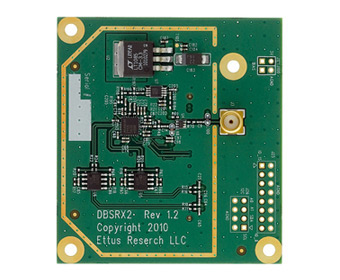
\includegraphics{Images/dbsrx2.jpg}
\isucaption{The DBSRX2 daughter board from Ettus Research (Image from Ettus Research Website - www.ettus.com)}
\label{dbsrx2}
\end{figure}
}

The DBSRX2 has several key components on it that is used to take the analog RF signal and prepare it for digitization by the analog to digital converter.  First the signal is amplified through a Programmable Gain Amplifier (PGA).  This PGA is accessible from the software and can be configured by the software.  Next the signal goes into a direct-conversion integrated circuit that directly converts the RF signal to analog I and Q values.  The integrated circuit, a Maxim MAX2112 device, also includes a Low Noise Amplifier (LNA), mixer and Low Pass Filter (LPF).  This essentially amplifies the signal, mixes into baseband and then applies a low pass filter.  

%{\begin{figure}[h!tb] 
%\centering
%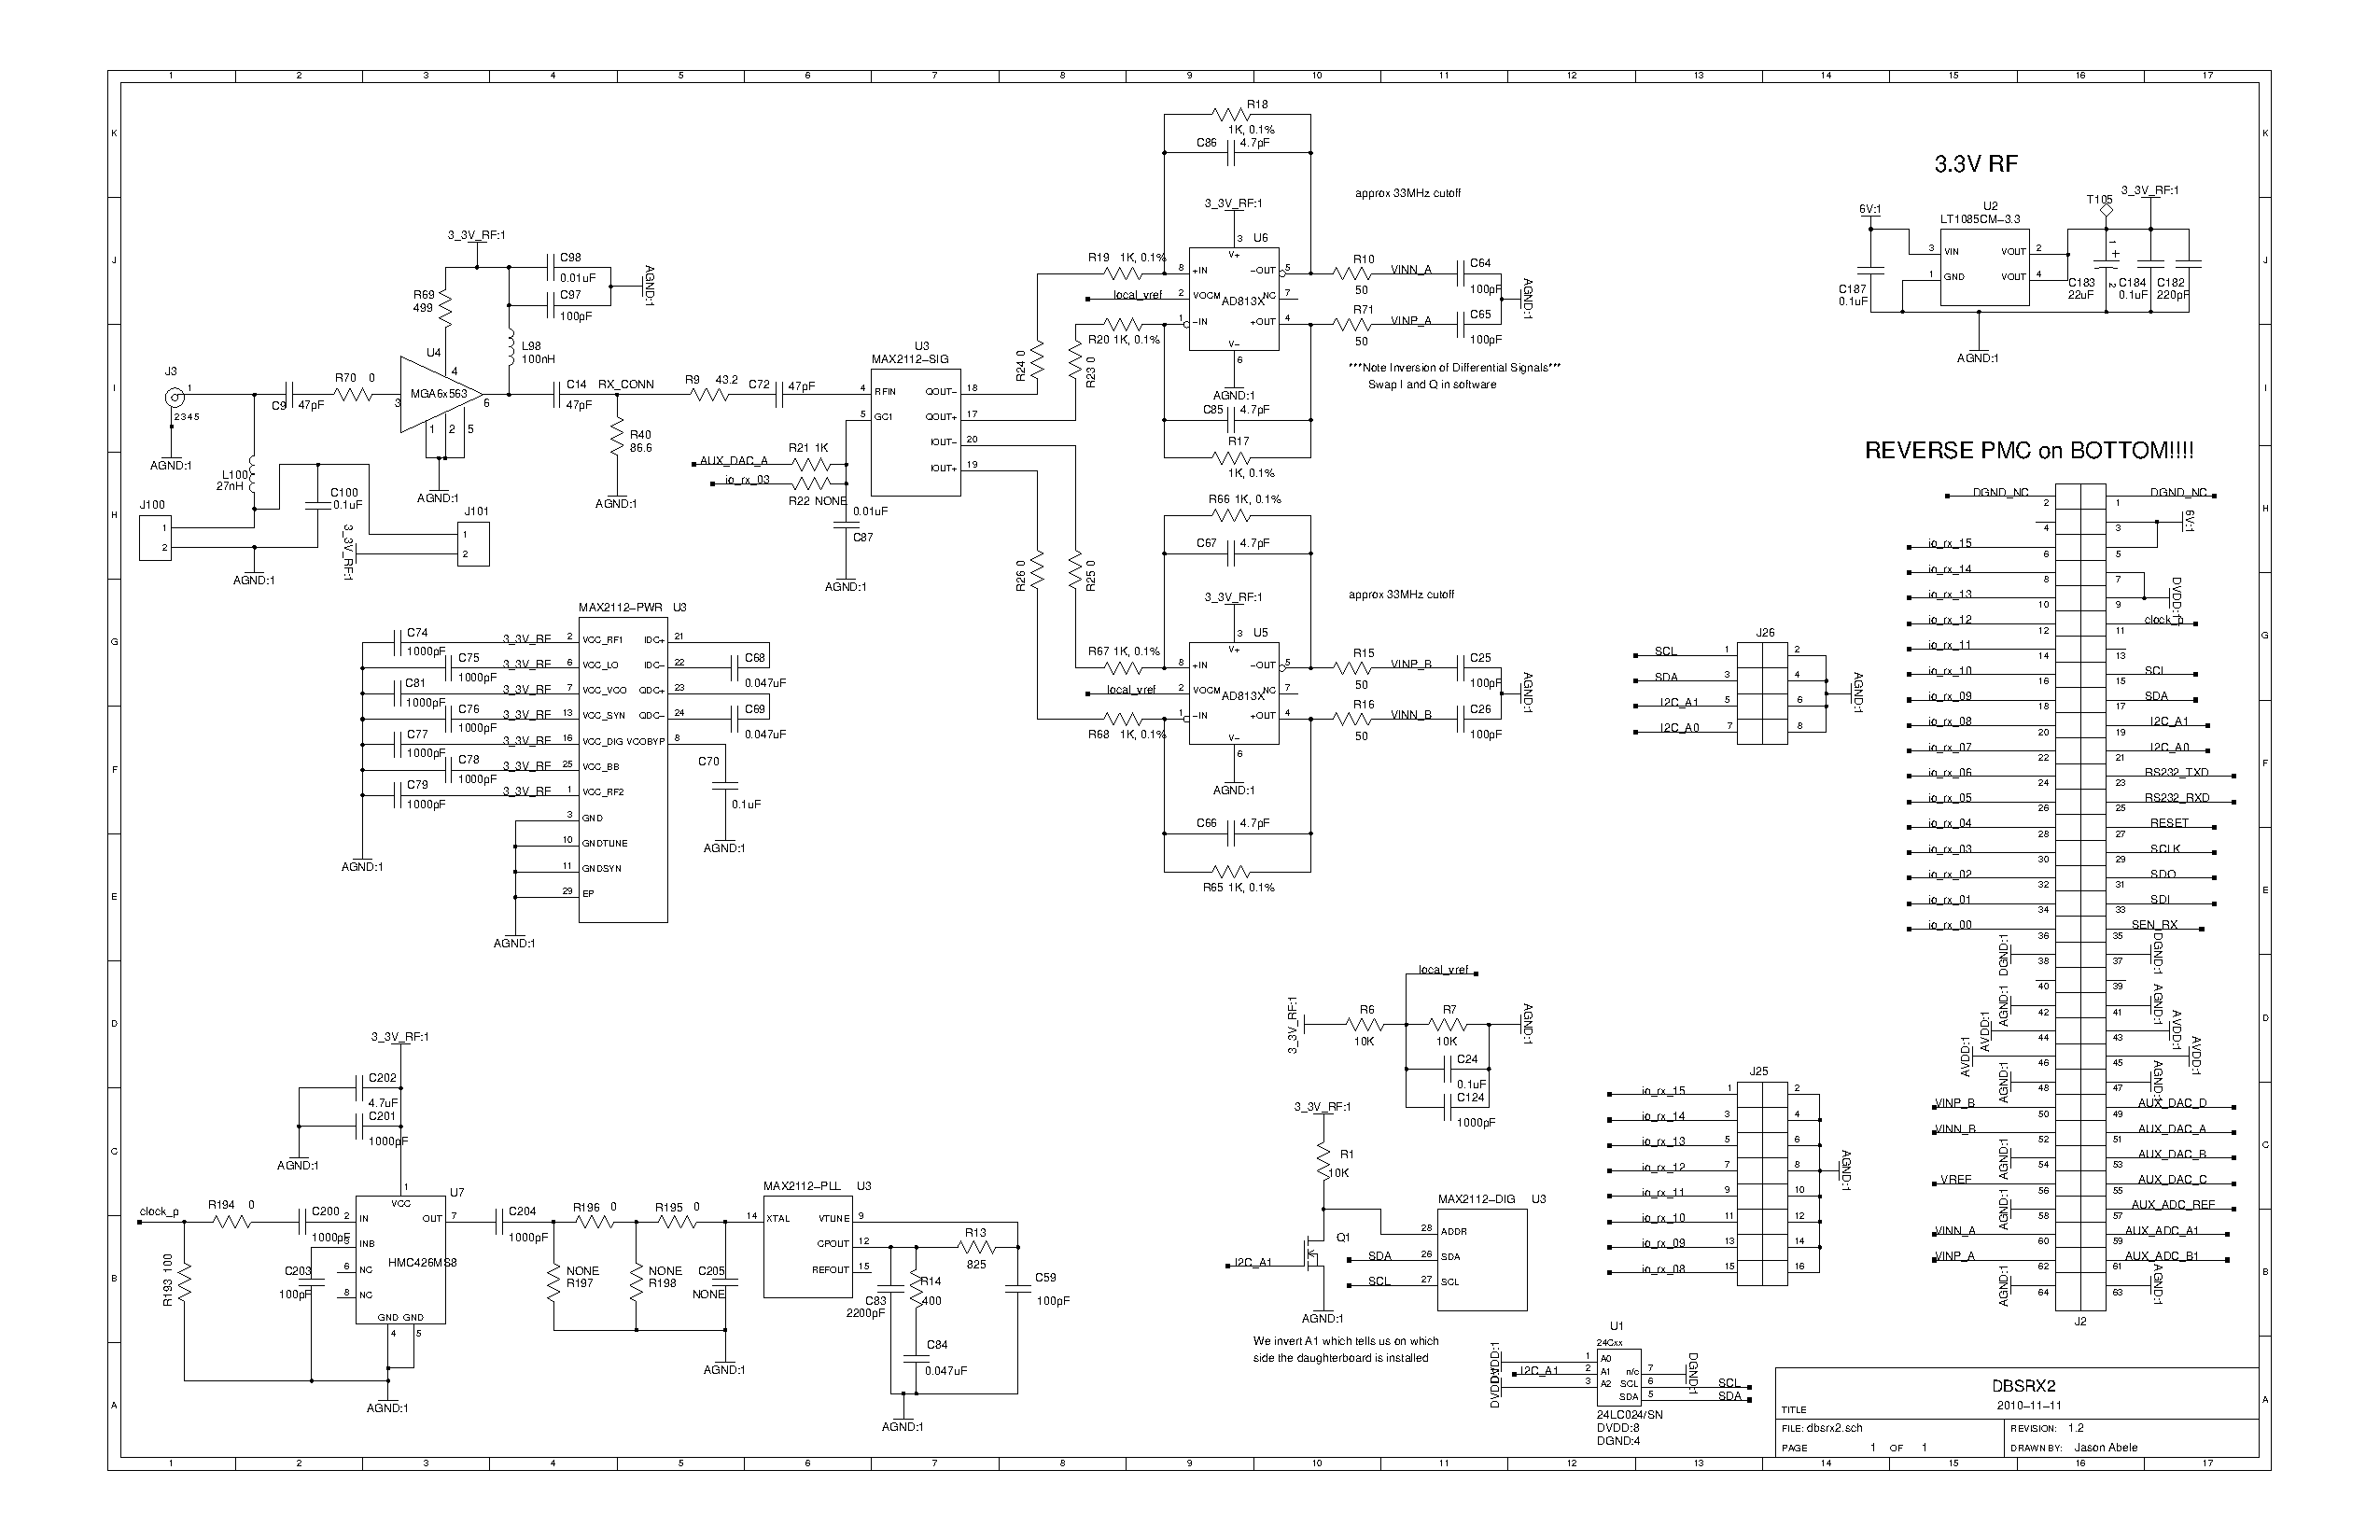
\includegraphics[width=\textwidth]{Images/dbsrx2.pdf}
%\isucaption{The DBSRX2 Schematic (Image from Ettus Research Website - www.ettus.com)}
%\label{dbsrx2_sch}
%\end{figure}
%}

These analog I and Q values are then passed to the N200 to be sampled by the analog to digital converter.  The IQ values are differential signals to minimize noise possible interference.

Since we are using the DBSRX2 after the LNAs that are already in use, the noise temperature added by the DBSRX2 will be small.  The DBSRX2 adds approximately 5 dB to the noise factor of the system.  Again though, since this is at the end of the RF chain, the total contribution of the DBSRX2 to the overall system noise temperature is small, and has been calculated to be 1.05 dB to the overall noise factor of the system.

\subsection{Software Platform} 

Software of course plays a critical role in a software defined radio and also in our software defined radio radiometer.  There are two pieces of software that are in play with the software defined radio we are using.  The first is the firmware that is used in the FPGA of the N200.  This firmware provides low level processing of the signal so it can be sent to the software located on the computer.  It also provides a link for controlling key aspects of the software defined radio such as additional gain, bandwidth and the center frequency.  This firmware is already pre-loaded into the FPGA by Ettus Research and can be upgraded through tools provided by Ettus Research.

The second is the software that is running on the host computer.  It is this software that provides the calculations on the I/Q data to give us the information we need and also creates a GUI for the user to interface with the radio.  For this software, we will be using GNURadio, an open source software program that is used in software defined radios including the N200 SDR that we have.  

GNURadio will be used to do all signal processing that is needed.  GNURadio is an open source software define radio framework that runs on multiple OSes and offers a rich set of features.  In addition, GNURadio is well supported by the Ettus Research group and is the preferred software for interfacing with their hardware.  

An easy to use interface was another driving requirement for our implementation of a radiometer in a SDR.  GNURadio helps us with this through the use of the GNU Radio Companion or GRC.  This was important as it was anticipated that operators of the radiometer have a limited knowledge about programming.  GRC uses a simple to use graphical system to design and build radio components in software.

%GNURadio  and GRC is written in Python, which allows for easy modification and access to additional tools that can be used with GNURadio.  While most of GNURadio is written in Python, C is used for any of the low level drivers and interface to the hardware.  This is done to optimize speed and performance of GNURadio.

%GNURadio fills in the software side of the software defined radio.  Although there is firmware that runs on the FPGA in the N200, this firmware is designed to communicate with a host PC.  It is this software that does most of the work by doing the calculations that apply to the signal.  The FPGA simply sends the raw IQ data to the host PC, which then performs the necessary math functions.  Again, the reason why software defined radios are desirable is the ability to change the behavior of the radio quickly.  In our scenario we can change functionality by simply loading a new software program in the host PC.  

%This functionality is ideal for communication type of radios where different modulation schemes and encoding and decoding methods can easily be changed out.  However, in a radiometer we are not interested in this aspect of the SDR.  However, one functionality is available that can be valuable for a radiometer, and that is with filtering.  Although we often use frequencies that should be free from interference, this is not always what happens in the real world.  Interference can and often does still occur, even in these protected frequencies.  With the SDR, we are able to quickly adapt to changing conditions by moving the frequency, changing our bandwidth and even filter out an offending signal.  

%GNURadio was selected as it is an open source software platform.  GNURadio is licensed under the GPL license and has a strong community that continually updates the software.  It is also well supported by third parties such as Ettus Research Group, National Instruments and other SDR developers.  In addition, GNURadio has a strong set of tools that can be used to develop programs that run under GNURadio.  Tools such as the GNURadio Companion (GRC) allows for an easy to use GUI to develop code for GNURadio.  GNURadio is also written in Python, which allows for easy modification and access to additional tools that can be used with GNURadio.  

{\begin{figure}[h!tb] 
\centering
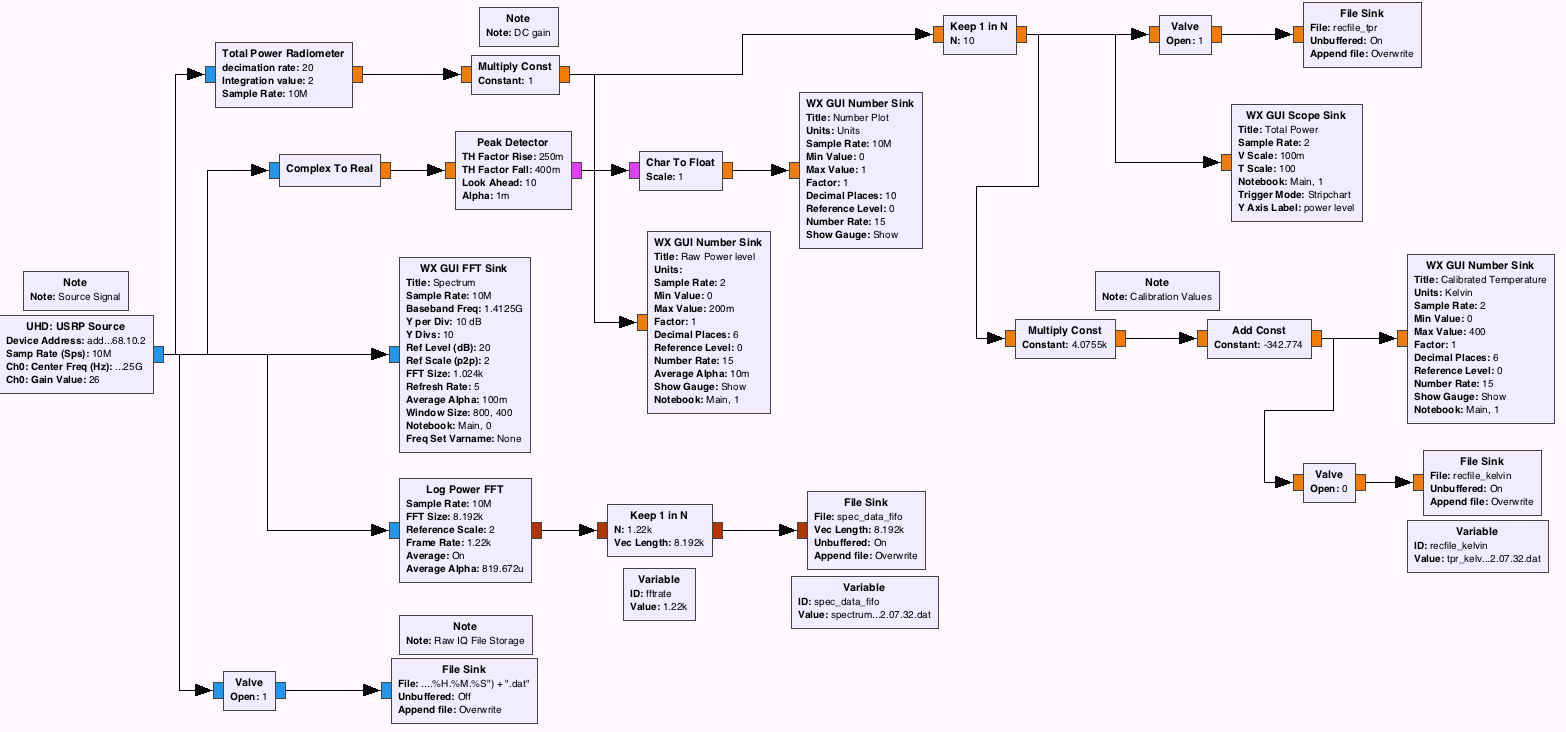
\includegraphics[width=17cm]{Images/N200_radiometer_grc.png}
\isucaption{Screenshot of the GNURadio Companion editor and the N200 Radiometer block diagram used in the author's experiments}
\label{N200_GRC}
\end{figure}
}

GNUradio Companion works by having the common functions as blocks that can picked and placed on the screen.  Once placed, the blocks can be wired up, much like LabView, and the flow of data can be controlled in this fashion.  While GNURadio Companion provides most of the essential blocks used in most applications additional blocks can by added if needed.  This is because GNURadio is built using Python and the blocks in GNUradio Companion are simply blocks of Python code.  To compile a GNURadio Companion flow diagram, you simply run the sheet, which then generates the Python code that is then executed.  

GNURadio uses a combination of Python and C++, where Python handles most of the interface and the C++ is most of the drivers and low level interface to the hardware.  This allows for an easy to use system but still meets the demanding performance needed for handling large amounts of data.  

GNURadio Companion also includes blocks that allow it to create a GUI type of interface.  The typical method it uses for this is using wxGUI although GNURadio Companion does also include blocks that can use QT for generating widgets as well.  However, the wxGUI tends to work better and has better support in GNURadio than QT.  

Through these blocks we are able to only manipulate the data we need to perform a total power radiometer in software but to also create a user interface that allows us to control the radiometer as well.  We are also able to display the information in real time so the user can see changes in power and even monitor spectral information during the operation of the radiometer. 


%----------------------------------------------------------
% End of Chapter 3.  Anything below this is extra information
